% !TEX program = pdflatex
% ============================================================
% Execution-Aware Portfolio RL (journal-style single-file manuscript)
% Single-file LaTeX (no external .bib required)
% Author: Kim Geum-Young
% ============================================================

\documentclass[10pt,twocolumn]{article}
\raggedbottom

% ---------- Page / Layout ----------
\usepackage[a4paper,margin=18mm]{geometry}
\usepackage{times}
\usepackage{microtype}

% ---------- Math / Theorems ----------
\usepackage{amsmath,amssymb,amsthm}
\newtheorem{proposition}{Proposition}
\newtheorem{lemma}{Lemma}
\newtheorem{corollary}{Corollary}
\newtheorem{remark}{Remark}

% ---------- Figures / Tables ----------
\usepackage{graphicx}
\usepackage{booktabs}
\usepackage{multirow}
\usepackage{array}
\usepackage{caption}
\usepackage{subcaption}
\usepackage{float}        % for [H]
\usepackage{dblfloatfix}  % improve placement of figure* / table* in twocolumn
\usepackage[section]{placeins}
\setlength{\textfloatsep}{8pt plus 1pt minus 2pt}
\setlength{\dbltextfloatsep}{8pt plus 1pt minus 2pt}
\setlength{\floatsep}{8pt plus 1pt minus 2pt}
\setlength{\intextsep}{8pt plus 1pt minus 2pt}

% ---------- Links ----------
\usepackage[hidelinks]{hyperref}

% ---------- Lists / Colors ----------
\usepackage{enumitem}
\usepackage{xcolor}

% ---------- Misc ----------
\usepackage{url}
\usepackage{authblk}

% ---------- Custom Macros ----------
\newcommand{\wexec}{w^{\mathrm{exec}}}
\newcommand{\wtgt}{w^{\mathrm{tgt}}}
\newcommand{\TOexec}{\mathrm{TO}^{\mathrm{exec}}}
\newcommand{\TOtgt}{\mathrm{TO}^{\mathrm{tgt}}}
\newcommand{\kappaTC}{\kappa}
\newcommand{\R}{\mathbb{R}}
\newcommand{\E}{\mathbb{E}}
\newcommand{\normone}[1]{\left\lVert #1 \right\rVert_1}
\newcommand{\normtwo}[1]{\left\lVert #1 \right\rVert_2}
\newcommand{\DeltaN}{\Delta^N}

% ---------- Title ----------
\title{\vspace{-6mm}
\textbf{Execution-Aware Portfolio Reinforcement Learning via Proximal Execution Control}\\
\vspace{-1mm}
\large Separating Target and Executed Portfolios for Cost-Aligned Evaluation and Execution Stabilization
\vspace{-3mm}
}
\author[1]{Kim Geum-Young}
\affil[1]{Chungbuk National University, Department of Software Engineering}
\date{}

\begin{document}

% ============================================================
% Title + Abstract across both columns (more journal-like)
% ============================================================
\twocolumn[{%
\maketitle
\vspace{-4mm}
\begin{abstract}
\vspace{-1mm}
Most portfolio reinforcement learning (RL) formulations treat the portfolio weights output by the policy as the portfolio that is immediately executed. Under transaction costs, this interface conflates target decisions with the realized holding path and obscures the object on which trading costs are actually incurred. We separate these objects through a two-stage decomposition: the policy outputs a target portfolio $\wtgt_t$, an execution controller produces an executed portfolio $\wexec_t$, and both transaction costs and primary evaluation are attached to executed turnover on the realized path. We evaluate this formulation in a frozen-policy, validation-first protocol that reuses one learned policy across all execution arms and changes only the execution rate $\eta$. On a fixed 27-name U.S. large-cap universe, the validation-selected interior operating point $\eta=0.5$ roughly halves executed turnover and improves net Sharpe in positive-cost regimes, while the $\kappa=0$ effect is negligible. The improvement is explained by lower realized turnover and lower realized cost rather than by higher gross returns, with rolling-window and friction-sensitivity diagnostics showing that the benefit is concentrated in positive-friction settings.
\end{abstract}

\vspace{-2mm}
\noindent\textbf{Keywords:} portfolio RL, transaction costs, execution, turnover, proximal control, reproducible backtesting
\vspace{1mm}
\hrule
\vspace{2mm}
}]

% ============================================================
\section{Introduction}
Portfolio RL is often formulated as if the portfolio weights output by the policy are the portfolio that is immediately held. This direct-action interface is convenient, but under transaction costs it collapses two different objects into one: the target portfolio proposed at decision time and the executed portfolio that is actually carried into the next return interval.

When execution is gradual, realized turnover, realized cost, and realized net return are determined by the executed path rather than by the raw target action alone. The distinction therefore matters even before one asks whether a different policy should be learned. It changes which portfolio is charged for trading costs, which return path is evaluated, and how one interprets the relation between portfolio choice and trade implementation.

The question studied here is therefore: under a fixed learned policy, does separating target and executed portfolios create an interior execution frontier in positive-cost regimes, and are the resulting net-performance changes explained by lower realized turnover and lower realized cost rather than by improved gross returns?

We adopt a frozen-policy protocol because retraining would change both the target generator and the execution interface at the same time. That joint comparison is important, but it answers a different question. Holding the learned policy fixed and varying only the execution mapping lets us identify how execution-aware accounting and partial execution affect realized net performance for the same learned target path.

\paragraph{Contributions.}
\begin{enumerate}[leftmargin=*,itemsep=2pt]
\item \textbf{Execution-aware portfolio interface and accounting.} We separate target and executed portfolios and attach transaction costs and primary evaluation to the realized executed path.
\item \textbf{Frozen-policy, validation-first identification protocol.} We evaluate one learned policy across fixed execution arms, select the operating point on validation only, and reserve the test window for held-out evaluation so that execution effects are separated from retraining effects.
\item \textbf{Friction-sensitive empirical evidence and diagnostics.} On the fixed 27-name U.S. large-cap benchmark, interior execution rates reduce turnover and improve net Sharpe in positive-cost regimes, and trace-based diagnostics show that the benefit comes from lower realized cost rather than higher gross returns.
\end{enumerate}
This paper does not propose a stronger portfolio policy. It isolates how execution-aware accounting and partial execution alone change realized net performance under frictions for a fixed learned policy.

% ============================================================
\section{Related Work}
\paragraph{Classical friction-aware portfolio choice.}
Classical portfolio theory studies dynamic allocation under risk/return trade-offs \cite{markowitz1952,merton1973}. Once trading frictions are introduced, however, the problem is no longer only which portfolio is desirable in isolation, but how current holdings should be adjusted toward that portfolio over time. Friction-aware portfolio optimization therefore shifts attention from static allocation to dynamic adjustment under transaction costs \cite{lobo2007,garleanu2013}.

\paragraph{Dynamic trading, aim portfolios, and partial adjustment.}
A closer conceptual predecessor is the dynamic-trading literature that separates current holdings from desired holdings and studies how portfolios move toward an aim portfolio under costs. G\^arleanu and Pedersen make that distinction explicit in a dynamic setting with predictable returns and transaction costs \cite{garleanu2013}. More broadly, this literature motivates partial adjustment and inaction-region reasoning once trading is costly. Our paper adopts the same basic separation, but relocates it into the portfolio-RL interface: the contribution is not a new frictional trading concept, but a re-specification of the accounting and evaluation object inside RL backtesting, where a learned target portfolio and the realized executed portfolio should not be conflated.

\paragraph{Optimal execution.}
Optimal-execution models also separate a desired position from the path used to reach it. Bertsimas and Lo and Almgren and Chriss study gradual trading that balances execution cost and risk, typically given an inventory objective or liquidation target \cite{bertsimas1998,almgren2000}. Our $\eta$-update is similar in implementation spirit to partial-adjustment rules from that literature, but the setting is different. We do not study an intraday execution optimizer. Instead, we study a daily execution layer that maps portfolio-policy outputs to executed holdings and changes how turnover, cost, and net performance are recorded for a fixed target path.

\paragraph{Portfolio RL, smoothing, and regularization.}
Most portfolio RL and deep portfolio management papers use a direct-action interface in which the policy output is treated as the portfolio that is immediately held or rebalanced to \cite{moody1998,jiang2017,ye2020}. Even when transaction costs are included, turnover is often computed directly from consecutive actions, so action turnover becomes a proxy for executed turnover. Related turnover-aware sequential-allocation work outside RL likewise studies frictions at the level of portfolio updates \cite{li2014}. Recent portfolio-RL variants improve robustness through richer state construction, auxiliary prediction, or reward shaping \cite{ye2020,lien2023}, and nearby RL work studies execution agents, hierarchical decomposition, or smooth-action regularization \cite{nevmyvaka2006,wang2021hrpm,shen2020,mysore2021}. The distinction in the present paper is therefore not simply ``smoother actions.'' It is that executed holdings are treated as the first-class accounting and evaluation object.

Taken together, the prior literature already contains gradual adjustment, aim portfolios, execution scheduling, and smoothing ideas. What is less explicitly isolated is a portfolio-RL experimental protocol in which target and executed portfolios are separated, primary evaluation is attached to the realized executed path, and the empirical effect of that separation is studied under a frozen learned policy. That narrower identification question is the one addressed here.

% ============================================================
\section{Problem Formulation}
\label{sec:setup}
We study an episodic daily portfolio-control problem over $N$ risky assets. The action space is the long-only fully invested simplex, there is no explicit cash asset, decisions are made once per trading day, and timing follows a close-to-close convention. At decision time $t$, the agent may use only information available up to close $t$; the portfolio held over $(t,t{+}1]$ is the executed portfolio formed after the decision at $t$.

We denote adjusted close prices by $p_t\in\R^N$. Single-period arithmetic returns over interval $(t,t{+}1]$ are
\[
r_{t+1} \triangleq \frac{p_{t+1}-p_t}{p_t}\in\R^N.
\]

\subsection{State}
At decision time $t$, the agent observes state $s_t$ constructed only from information available up to time $t$. In the empirical instantiation, $s_t$ contains a rolling return window, per-asset volatility estimates, previous executed weights, and optional frozen signal channels; Section~\ref{sec:exp} gives the exact window lengths and feature counts.

\subsection{Action}
The policy outputs a target portfolio $\wtgt_t=\pi_\theta(s_t)$ in the long-only fully invested simplex
\[
\DeltaN \triangleq \{w\in\R^N_+:\mathbf{1}^\top w=1\}.
\]
Thus the MDP action is a \emph{target} portfolio rather than the realized holding vector. In the empirical implementation, the actor emits unconstrained real-valued logits that are mapped into $\DeltaN$ by a stable softmax; Section~\ref{sec:exp} records that concrete parameterization.

\subsection{Execution Mapping}
Let the previous executed portfolio be $\wexec_{t-1}$. The execution layer maps the target portfolio to an executed portfolio according to
\begin{align}
\wtgt_t &= \pi_\theta(s_t)\in\DeltaN, \label{eq:tgt_policy}\\
\wexec_t &= (1-\eta_t)\wexec_{t-1} + \eta_t \wtgt_t,\quad \eta_t\in(0,1], \label{eq:exec_update}\\
\TOtgt_t &= \normone{\wtgt_t - \wexec_{t-1}}, \label{eq:turnover_tgt}\\
\TOexec_t &= \normone{\wexec_t - \wexec_{t-1}}. \label{eq:turnover_exec}
\end{align}
Here $\TOtgt_t$ is the turnover implied by an immediate move to the target portfolio, while $\TOexec_t$ is the turnover actually realized on the executed path.

\subsection{Reward and Realized Return}
Transaction costs are charged on executed turnover, and realized reward is attached to the executed portfolio:
\begin{align}
\mathrm{cost}_{t} &= \kappaTC \, \TOexec_t, \label{eq:cost_exec}\\
R_{t+1} &= (\wexec_t)^\top r_{t+1} - \mathrm{cost}_t, \label{eq:reward}\\
R^{\mathrm{tgt}}_{t+1} &= (\wtgt_t)^\top r_{t+1} - \kappaTC \TOtgt_t. \label{eq:reward_tgt_diag}
\end{align}
The quantity $R_{t+1}$ is the realized executed-path return used for primary evaluation. The quantity $R^{\mathrm{tgt}}_{t+1}$ is a hypothetical target-path return used only for diagnostics. The MDP action is therefore $\wtgt_t$, while realized portfolio dynamics and primary reward are governed by the executed path $\wexec_t$ and \eqref{eq:reward}.

\subsection{Terminology and Evaluation Objects}
Throughout the paper, \emph{target portfolio} denotes the policy output $\wtgt_t$, \emph{executed portfolio} denotes the realized holdings $\wexec_t$, \emph{immediate-execution baseline} denotes the comparison arm $\eta=1.0$, \emph{validation-selected operating point} denotes the execution rate chosen on the validation window, and \emph{net Sharpe} denotes the annualized Sharpe ratio computed from executed net linear returns. The code label \texttt{sharpe\_net\_lin} is the implementation name for this same net-Sharpe quantity.

\begin{table}[t]
\centering
\scriptsize
\caption{Core versus diagnostic quantities.}
\label{tab:core_vs_diag}
\begin{tabular}{@{}lll@{}}
\toprule
Quantity & Role & Primary evaluation \\
\midrule
$\TOtgt_t$ & target-turnover diagnostic & No \\
$\TOexec_t$ & executed turnover & Yes \\
$R^{\mathrm{tgt}}_{t+1}$ & hypothetical target-path return & No \\
$R_{t+1}$ & realized executed-path return & Yes \\
$\normtwo{\wexec_t-\wtgt_t}$ & tracking diagnostic & No \\
\bottomrule
\end{tabular}
\end{table}

Primary portfolio metrics such as Sharpe, CAGR, and max drawdown are computed from the realized executed-path returns $\{R_{t+1}\}$. Diagnostics may additionally use $\wtgt_t$, $\TOtgt_t$, $R^{\mathrm{tgt}}_{t+1}$, or target--executed tracking discrepancies, but these objects are explicitly labeled and never serve as the primary evaluation metric.

% ============================================================
\section{Execution-Aware Control and Accounting}
This section defines the execution-aware interface and the frozen-policy accounting protocol used throughout the experiments. The theoretical section that follows is narrower: it records simple analytical properties of the execution map that help interpret the empirical results without overstating the depth of the theory contribution.
\subsection{Two-stage control}
We interpret portfolio RL under frictions as a two-stage control problem:
\begin{enumerate}[leftmargin=*,itemsep=1pt]
\item \textbf{Policy layer:} the agent chooses a desired allocation $\wtgt_t=\pi_\theta(s_t)$.
\item \textbf{Execution layer:} the controller maps that desired allocation into realized holdings $\wexec_t$ via \eqref{eq:exec_update}.
\end{enumerate}
The formulation naturally supports learning under the executed dynamics \eqref{eq:reward}. In the present empirical study, however, the policy layer is trained exactly once and then held fixed; every empirical arm reuses that same trained policy and varies only the execution layer. The resulting comparison isolates how execution-aware accounting changes realized performance for the same learned target path.

\subsection{Fixed execution timescale}
The execution update \eqref{eq:exec_update} is fixed, and the present paper studies only constant timescales $\eta_t\equiv\eta$. This is an identification choice rather than only a simplification. Once $\eta_t$ becomes rule-based or learned, the object of study shifts from execution accounting to adaptive controller design. Fixed $\eta$ removes schedule-design confounds and keeps the empirical question at the level of how partial execution alone changes realized turnover, realized cost, and net performance.

\subsection{Cost alignment (core principle)}
Cost should be attached to what is actually traded, not to what was merely proposed. The primary accounting object is therefore executed turnover $\TOexec_t$ and the realized executed-path return \eqref{eq:reward}. Target-based cost and target-path return remain useful as counterfactual diagnostics, but they are not the primary accounting object because they describe a hypothetical immediate move that was not actually executed. Charging costs on target turnover $\TOtgt_t$ induces systematic friction mis-scaling when $\eta_t<1$ (Proposition~\ref{prop:cost_misalignment}); the present paper studies that accounting implication under a frozen-policy protocol rather than running alternative retraining experiments.

% ============================================================
\section{Theoretical Analysis}
\label{sec:theory}
This section collects simple analytical properties needed for interpretation: the proximal form of the update, realized-turnover scaling, tracking and low-pass behavior, and the accounting distortion induced by target-based cost charging.

\begin{proposition}[Proximal interpretation]\label{prop:prox}
For constant $\eta\in(0,1)$, the execution update \eqref{eq:exec_update} is the unique minimizer of:
\[
\begin{aligned}
\wexec_t=\arg\min_{w \in \DeltaN}\;
&\frac{1}{2}\normtwo{w-\wexec_{t-1}}^2 \\
&+ \frac{\eta}{2(1-\eta)}\normtwo{w-\wtgt_t}^2.
\end{aligned}
\]
\end{proposition}
\noindent\textbf{Proof sketch.} The objective is strongly convex in $w$. Setting the gradient to zero yields a convex combination of $\wexec_{t-1}$ and $\wtgt_t$; the simplex constraint is preserved by convexity of $\DeltaN$. \hfill$\square$
\begin{remark}
Execution is a proximal step that penalizes \emph{changes from the previous executed portfolio}, regularizing the trading path while still tracking the target.
\end{remark}

\begin{lemma}[Turnover scaling and cumulative bound]\label{lem:turnover_scaling}
Under \eqref{eq:exec_update}--\eqref{eq:turnover_exec}, for any $\eta_t\in(0,1]$:
\[
\TOexec_t = \eta_t \TOtgt_t.
\]
If additionally $\eta_t\le \eta_{\max}$ for all $t$, then
\[
\sum_{t=1}^T \TOexec_t \le \eta_{\max}\sum_{t=1}^T \TOtgt_t.
\]
\end{lemma}
\noindent\textbf{Proof sketch.} From \eqref{eq:exec_update},
$\wexec_t-\wexec_{t-1}=\eta_t(\wtgt_t-\wexec_{t-1})$.
Taking $\ell_1$ norms gives the one-step identity. Summing over $t$ and using $\eta_t\le \eta_{\max}$ yields the cumulative bound. \hfill$\square$

\begin{lemma}[Tracking and low-pass behavior]\label{lem:tracking_lowpass}
Define instantaneous tracking discrepancy by $\normtwo{\wexec_t-\wtgt_t}$. Then
\[
\wexec_t-\wtgt_t = (1-\eta_t)(\wexec_{t-1}-\wtgt_t),
\]
so for fixed $(\wexec_{t-1},\wtgt_t)$, smaller $\eta_t$ increases discrepancy whenever $\wexec_{t-1}\neq \wtgt_t$.
For constant $\eta\in(0,1]$, the executed sequence has the closed form:
\[
\wexec_t = (1-\eta)^t \wexec_0 + \eta\sum_{i=1}^{t} (1-\eta)^{t-i}\wtgt_i.
\]
For fixed horizon $t$, $\eta\to0$ implies $\wexec_t\to \wexec_0$ (anchor convergence).
\end{lemma}
\noindent\textbf{Proof sketch.} Rearranging \eqref{eq:exec_update} yields the tracking identity. Unrolling the constant-$\eta$ recursion yields the closed form, which is an exponential smoothing of the target path. \hfill$\square$

\begin{proposition}[Cost misalignment rescaling]\label{prop:cost_misalignment}
If one incorrectly charges costs using target turnover $\TOtgt_t$ while execution obeys \eqref{eq:exec_update}, then the charged cost overestimates realized cost by factor $1/\eta_t$:
\[
\kappaTC \TOtgt_t \;=\; \frac{\kappaTC}{\eta_t}\TOexec_t.
\]
Equivalently, the target-based cost distortion is
\[
\begin{aligned}
\kappaTC \TOtgt_t - \kappaTC \TOexec_t
&= \kappaTC(\TOtgt_t-\TOexec_t) \\
&= \kappaTC\left(\frac{1}{\eta_t}-1\right)\TOexec_t.
\end{aligned}
\]
\end{proposition}
\noindent\textbf{Proof sketch.} Substitute Lemma~\ref{lem:turnover_scaling} into $\kappaTC\TOtgt_t$ and subtract the executed cost term. \hfill$\square$

\noindent\textbf{Interpretation.} Target-based charging inflates the effective friction scale whenever $\eta_t<1$. If that target-based cost is inserted into training rewards, the friction coefficient appearing in critic targets and policy updates is larger than the one actually realized on the executed path. The present paper does not quantify full policy-gradient bias or retrain under alternative rewards; it records the accounting distortion and its direction.

These properties are simple but useful: they clarify what quantity is actually being regularized, what turnover is actually realized, and how target-based accounting distorts the friction scale when $\eta<1$.

% ============================================================
\section{Experimental Setup}
\label{sec:exp}

\subsection{Data, universe, and splits}
We use a fixed 27-name large-cap U.S. equity snapshot with daily adjusted close prices retrieved via \texttt{yfinance}. The frozen-control study uses:
\begin{itemize}[leftmargin=*,itemsep=1pt]
\item Train window: 2010-01-01 to 2021-12-31.
\item Validation window: 2022-01-01 to 2023-12-31.
\item Test window: 2024-01-01 to 2025-12-31.
\item Decision frequency: daily rebalancing.
\end{itemize}
Because the state uses 30-day rolling features, the realized validation trace spans 2022-02-15 to 2023-12-29 and the realized held-out test trace spans 2024-02-14 to 2025-12-31. Matched external baselines are evaluated on these same effective held-out dates.
Timing follows a close-to-close convention: features at time $t$ use information available by close $t$, the execution update forms $\wexec_t$ after the decision at $t$, and realized portfolio return uses $r_{t+1}$ over $(t,t+1]$. This fixed 27-name large-cap U.S. equity snapshot is reproducible but not a point-in-time constituent reconstruction, so the empirical claims should be read as controlled benchmark evidence rather than as a survivorship-bias-free deployment backtest. Survivorship-related bias may affect the absolute performance level. Because all $\eta$-arms share the same universe, dates, and frozen target policy, the within-policy execution comparison is less sensitive to this bias than absolute cross-strategy comparisons, though it is not immune. Internal 2026 forward checks were used for engineering sanity only and are not part of the main paper tables. Appendix~\ref{app:data_protocol} collects the data and protocol details in one place for auditability.

\subsection{Observations and environment}
The empirical instantiation uses a 30-day return window ($L=30$), a 30-day volatility window ($L_v=30$), previous executed weights $\wexec_{t-1}$, and two frozen signal channels: \texttt{reversal\_5d} and \texttt{short\_term\_reversal}. The return block stores flattened per-asset log returns computed from adjusted-close ratios. The volatility block stores the 30-day rolling standard deviation (ddof $=0$) of those same log returns. The previous-weight block stores the simplex-valued executed holdings from time $t-1$, and the signal channels are appended in the same asset order. For the fixed 27-asset universe, this yields $30\times27 + 27 + 27 + 2\times27 = 918$ observation dimensions, matching the stored run metadata.

No additional online whitening or environment-level normalization is applied beyond the upstream feature construction. Realized portfolio return is evaluated on arithmetic returns obtained from the stored log-return frame, and anti-lookahead is enforced by forming $s_t$ only from information available up to time $t$ and applying $\wexec_t$ to interval return $r_{t+1}$.

The actor outputs a 27-dimensional real-valued action vector. In the environment, that vector is clipped elementwise to $[-1,1]$ and mapped to long-only fully invested target weights by a stable softmax with logit scale 10.0. This implementation detail matters because it makes the simplex constraint operational: the learned action parameterization always produces a valid target portfolio before the execution layer is applied.

\subsection{Frozen controller and execution arms}
\begin{itemize}[leftmargin=*,itemsep=1pt]
\item \textbf{PRL-SAC control model:} a Stable-Baselines3 SAC controller with an \texttt{MlpPolicy} actor-critic backbone and volatility-conditioned PRL plasticity schedule. For each seed, the controller is trained once on the training window, producing one frozen checkpoint. Evaluation then reuses that same checkpoint across all $\eta$-arms for that seed. The policy outputs target-allocation logits; the environment maps them to simplex weights before the execution layer applies partial adjustment. The exact training hyperparameters and frozen scheduler settings are summarized in Appendix~\ref{app:implementation_details}.
\item \textbf{Execution-control arms:} the same trained policy is evaluated under the \emph{a priori} fixed grid $\eta\in\{1.0, 0.5, 0.2, 0.1, 0.082, 0.05, 0.02\}$, with $\eta=1.0$ as the immediate-execution baseline.
\end{itemize}

\subsection{Internal comparison arms}
The main comparison in this paper is internal and isolates execution while holding the learned controller fixed:
\begin{itemize}[leftmargin=*,itemsep=1pt]
\item \textbf{Immediate-execution baseline:} fixed $\eta=1.0$.
\item \textbf{Execution-aware variants:} the interior $\eta$ values from that same fixed grid.
\end{itemize}
This design keeps the predictive model constant and attributes performance differences to execution alone. Matched external heuristics are handled separately so that the main causal comparison remains ``same frozen policy, different execution rule,'' while non-RL reference portfolios are added only under the same accounting conventions.

\subsection{Transaction cost regimes}
Sweep $\kappaTC\in\{0,\;5\times10^{-4},\;10^{-3}\}$ and evaluate the fixed $\eta$ grid with paired seeds.

\subsection{A priori \texorpdfstring{$\eta$}{eta} grid and validation-only selection}
\label{sec:validation_selection}
The $\eta$ grid is fixed before evaluation and is not adapted after looking at test outcomes. It combines the immediate-execution boundary $\eta=1.0$, coarse interior values $\{0.5,0.2,0.1\}$, and finer low-$\eta$ probes $\{0.082,0.05,0.02\}$ to inspect frontier curvature in the low-adjustment region. The value $\eta=0.082$ is included because it is the incumbent \texttt{rebalance\_eta} of the frozen control snapshot used to train the reference policy; it is therefore a pre-existing control operating point rather than a post-hoc addition after inspecting validation or test performance. Let the positive-cost validation set be $\mathcal{K}^{+}=\{5\times10^{-4},10^{-3}\}$. For each $\eta$ in the fixed grid, we define the validation score
\[
\mathrm{Score}(\eta)\triangleq \frac{1}{|\mathcal{K}^{+}|}\sum_{\kappa\in\mathcal{K}^{+}}\mathrm{median}_{s\in\mathcal{S}}\;\mathrm{Sharpe}^{\mathrm{net,lin}}_{\kappa,\eta,s}.
\]
We then select the \emph{largest} $\eta$ satisfying
\[
\mathrm{Score}(\eta)\;\ge\;\tau(b),\qquad
b\triangleq \max_{\eta'} \mathrm{Score}(\eta'),
\]
with the signed relative threshold
\[
\tau(b)\triangleq
\begin{cases}
0.95\,b, & b>0,\\
b/0.95, & b<0,\\
0, & b=0.
\end{cases}
\]
Thus, $\eta$ selection is based on the validation window only and intentionally favors the least aggressive execution smoothing among near-best validation operating points. The 2024--2025 test window is used only for final held-out evaluation of the selected operating point and is never used for $\eta$ selection.

\subsection{Evaluation protocol (paired seeds)}
Let $\mathcal{S}=\{0,1,\dots,9\}$. For each seed $s\in\mathcal{S}$, evaluate all arms (different $\eta$ values) with identical data splits and the same frozen trained policy per seed.
Report:
\begin{itemize}[leftmargin=*,itemsep=1pt]
\item Median across seeds for each reported metric in the main tables.
\item Paired differences (e.g., $\Delta$Sharpe) and win-rate (\% seeds improved) versus the immediate-execution baseline $\eta=1.0$.
\item For the selected-$\eta$ vs.\ immediate-execution comparison, also report paired dispersion (IQR), exact one-sided sign-test $p$-values, two-sided Wilcoxon signed-rank $p$-values, and percentile-bootstrap $95\%$ confidence intervals for the paired median $\Delta$Sharpe and $\Delta$CAGR.
\end{itemize}
These seed-level tests quantify optimization-level variability conditional on a fixed historical window, not independent market-sample uncertainty.

\subsection{Secondary matched-heuristic context under aligned definitions}
To provide limited non-RL context without changing the main question, the rebuilt protocol also includes five heuristic baselines on the same effective held-out dates within the test split: buy-and-hold equal weight, daily-rebalanced equal weight, inverse-volatility risk parity, minimum-variance, and a simple long-only mean-variance heuristic. The two optimization-style heuristics use a trailing 252-day window with a minimum 30-day warm-up, and the mean-variance heuristic fixes risk aversion at 10.0. These baselines are not allowed to use a different accounting convention. They must use the same transaction-cost regime $\kappaTC$, the same realized-path net-return definition, the same Sharpe annualization $\sqrt{252}$, the same risk-free assumption $r_f=0$, the same executed-path primary metric definitions as the RL arms, and the same effective evaluation dates induced by the frozen split and rolling-feature availability. They are included only to calibrate external performance scale under aligned accounting. They are not part of the identification strategy, and they are not used for selection, validation, or the paper's core causal interpretation.

\subsection{Metrics}
\paragraph{Core metrics (exec only).}
Sharpe, CAGR, max drawdown, average executed turnover $\overline{\TOexec}$, and realized cost are computed from the executed-path quantities in Table~\ref{tab:core_vs_diag}. Specify annualization and risk-free assumption:
\begin{itemize}[leftmargin=*,itemsep=1pt]
\item Sharpe annualization: $\sqrt{252}$.
\item Risk-free rate: 0.
\end{itemize}
These same definitions are used for both RL arms and external heuristic baselines.

\paragraph{Diagnostics (target used for analysis only).}
\begin{itemize}[leftmargin=*,itemsep=1pt]
\item Target turnover $\overline{\TOtgt}$.
\item Tracking error / misalignment measures (defined below).
\end{itemize}

\paragraph{Diagnostic path comparisons.}
Using the diagnostic target-path return $R^{\mathrm{tgt}}_{t+1}$ from Section~\ref{sec:setup}, we compute path-space comparisons between the realized executed path and the hypothetical immediate target path. A signed mean-gap diagnostic can then be written as
\[
\Delta_{\mathrm{mis}} \triangleq \frac{1}{T}\sum_{t=0}^{T-1}\left(R_{t+1} - R^{\mathrm{tgt}}_{t+1}\right).
\]
In our runs, this signed average is numerically small and less informative than path-space quantities. The main paper therefore emphasizes trace-based absolute diagnostics:
\begin{itemize}[leftmargin=*,itemsep=1pt]
\item mean absolute return gap $\frac{1}{T}\sum_t |R_{t+1}-R^{\mathrm{tgt}}_{t+1}|$,
\item final equity gap $|E_T^{\mathrm{exec}}-E_T^{\mathrm{tgt}}|$,
\item maximum daily absolute gap $\max_t |R_{t+1}-R^{\mathrm{tgt}}_{t+1}|$,
\item average weight-path tracking discrepancy.
\end{itemize}

% ============================================================
\section{Results}
\label{sec:results}

\subsection{Protocol framing: validation selection, then held-out evaluation}
The empirical protocol is two-stage. First, the fixed $\eta$ grid is scored on the validation window and one operating point is selected using the rule from Section~\ref{sec:validation_selection}. Second, the held-out test window is used only for final evaluation of that validation-selected operating point and the immediate-execution baseline. No test statistic is used to choose $\eta$. Every result in this section reuses the same trained policy and changes only the execution mapping applied to that frozen target path. The main paper evidence is therefore organized around: (i) a validation frontier plus selection report, (ii) a held-out selected-$\eta$ vs.\ $\eta=1.0$ table, (iii) trace-based mechanism diagnostics, (iv) a rolling-window frontier robustness diagnostic, and (v) a denser canonical friction-grid diagnostic. The full held-out $\eta$ frontier is still useful, but only as a post-selection diagnostic rather than as model-selection evidence. A small matched-heuristic comparison is retained in the appendix only as secondary context. In the rolling-window extension reported later in this section, the distinction between selected-point transfer and frontier robustness becomes especially important: the selected operating point is window-sensitive, whereas the positive-cost held-out frontier itself is more stable.

\subsection{Validation selection locks the operating point at \texorpdfstring{$\eta=0.5$}{eta=0.5}}
Table~\ref{tab:validation_selection} reports the validation-only selection object. All positive-cost validation scores are positive in this rebuilt run, so the selection problem is about taking the largest $\eta$ that remains close to the best validation frontier point. The raw best validation score is attained at $\eta=0.02$ with $0.5213$, but the locked $95\%$ rule qualifies six interior grid points and then selects the \emph{largest} qualifying value. The resulting validation-selected operating point is therefore $\eta=0.5$, while the immediate-execution baseline $\eta=1.0$ narrowly fails the qualification threshold.

This matters for interpretation. The main empirical claim is no longer that one hand-picked small $\eta$ looks attractive on test, but that a validation-selected interior operating point transfers to the held-out window without using test outcomes for model selection. Because the trained policy is held fixed throughout, this is an execution-choice result rather than a retraining result. A small threshold-sensitivity check also supports the rule itself: tightening the relative threshold from $95\%$ to $97.5\%$ still selects $\eta=0.5$, whereas only the looser $90\%$ rule reverts to $\eta=1.0$. Relative to the raw best point $\eta=0.02$, the locked choice $\eta=0.5$ retains $97.66\%$ of the best validation score while keeping average positive-cost tracking error much smaller ($0.00257$ versus $0.00692$). Validation also already shows the turnover mechanism clearly: seed-median executed turnover falls from $0.02160$ at $\eta=1.0$ to $0.01087$ at $\eta=0.5$, a reduction of about $49.7\%$. Figure~\ref{fig:frontier} visualizes this validation result.

\begin{table*}[t]
\centering
\scriptsize
\caption{Validation-only $\eta$ selection on the 2022--2023 split. Let $\kappa^+=\{5\times10^{-4},10^{-3}\}$. The score is the mean, over $\kappa\in\kappa^+$, of the seed-median net Sharpe. The selected operating point is the largest $\eta$ within the locked relative threshold of the best validation score.}
\label{tab:validation_selection}
\begin{tabular}{@{}rrrrrr@{}}
\toprule
$\eta$ & Score & Avg.\ paired-median $\Delta$Sharpe ($\kappa>0$) & Avg.\ seed-median executed turnover ($\kappa>0$) & Qualifies & Selected \\
\midrule
0.500 & 0.50907 & 0.01409 & 0.01087 & Yes & Yes \\
0.200 & 0.51359 & 0.02290 & 0.00501 & Yes & No \\
0.100 & 0.51704 & 0.02678 & 0.00271 & Yes & No \\
0.082 & 0.51791 & 0.02768 & 0.00226 & Yes & No \\
0.050 & 0.51958 & 0.02919 & 0.00143 & Yes & No \\
0.020 & 0.52126 & 0.03093 & 0.00060 & Yes & No \\
1.000 & 0.49327 & 0.00000 & 0.02160 & No & No \\
\bottomrule
\end{tabular}
\end{table*}

\begin{figure*}[t!]
\centering
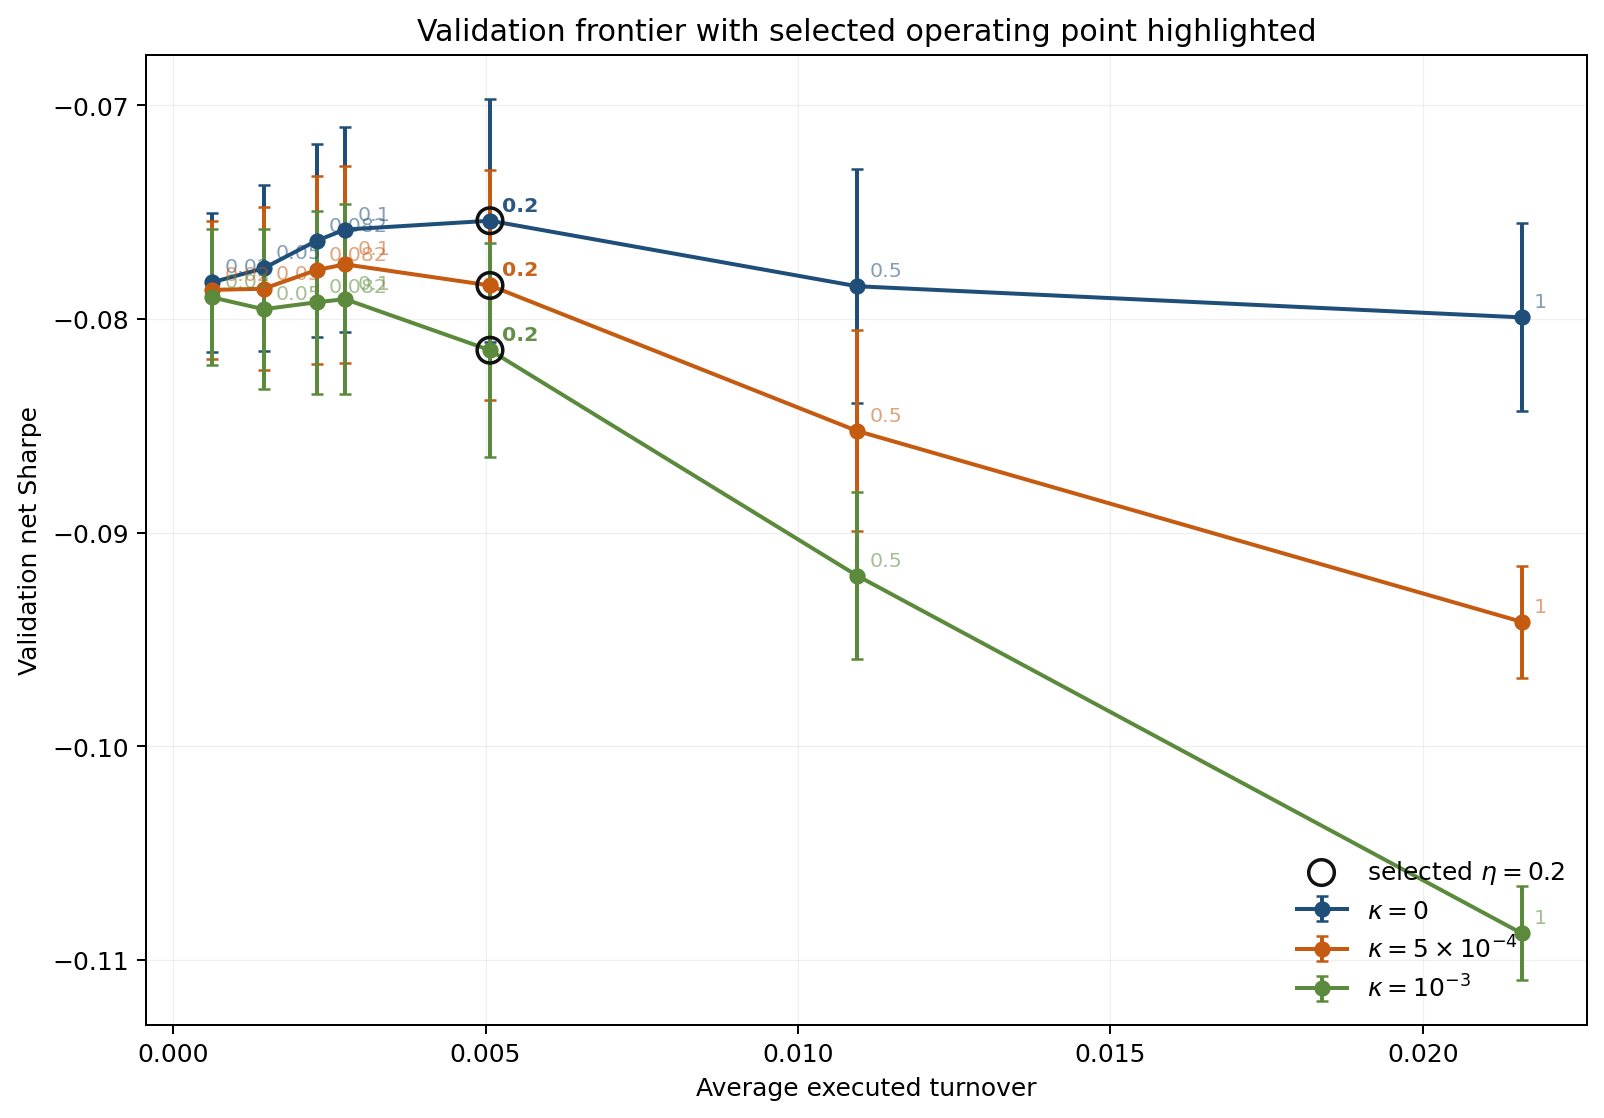
\includegraphics[width=0.95\textwidth]{fig_frontier.png}
\caption{Validation frontier on the effective validation dates 2022-02-15 to 2023-12-29 within the 2022--2023 split. Each colored line corresponds to one transaction-cost regime $\kappa\in\{0,5\times10^{-4},10^{-3}\}$, and each labeled point is one $\eta$ value. Horizontal position is seed-median executed turnover across the 10 validation seeds, vertical position is the median net Sharpe, and vertical bars show half-IQR of seedwise net Sharpe. The validation-selected operating point $\eta=0.5$ is emphasized with enlarged black-edged markers.}
\label{fig:frontier}
\end{figure*}

\subsection{Held-out test: selected \texorpdfstring{$\eta=0.5$}{eta=0.5} vs.\ immediate execution}
Table~\ref{tab:selected_vs_eta1} gives the held-out paired comparison between the validation-selected operating point and the immediate-execution baseline. The main evidence is again concentrated in the positive-cost regimes. At $\kappa=5\times10^{-4}$ and $\kappa=10^{-3}$, the selected operating point improves paired median net Sharpe by $+0.0105$ and $+0.0213$, respectively, and wins on all $10/10$ paired seeds in both cases (exact one-sided sign test $p=9.77\times10^{-4}$ for each regime). The corresponding two-sided Wilcoxon signed-rank $p$-values are $1.95\times10^{-3}$ in both regimes, and the bootstrap $95\%$ confidence intervals for the paired median $\Delta$Sharpe remain strictly positive: $[0.0073,\,0.0129]$ at $\kappa=5\times10^{-4}$ and $[0.0167,\,0.0233]$ at $\kappa=10^{-3}$. Median executed turnover falls from $0.02200$ to $0.01095$ in all three reported rows, roughly halving executed trading intensity.

At $\kappa=0$, the picture is negligible. The paired median Sharpe delta is $-0.00025$ with a $50\%$ win-rate, sign-test $p=0.623$, Wilcoxon $p=0.770$, and a bootstrap $95\%$ confidence interval of $[-0.0022,\,0.0028]$ for the paired median $\Delta$Sharpe. This is consistent with little difference in the realized trading path once explicit transaction costs are removed, and it does not support a strong regularization or training-superiority interpretation. The regime contrast is therefore clear: evidence is strong for cost-aligned improvement when $\kappaTC>0$, and absent when $\kappaTC=0$. Because the first two Sharpe columns report marginal arm medians while $\Delta$Sharpe reports the median of seed-wise paired differences, the paired median need not equal the arithmetic difference between the two marginal medians.

\begin{table*}[t]
\centering
\scriptsize
\caption{Held-out test comparison between the validation-selected operating point $\eta=0.5$ and the immediate-execution baseline $\eta=1.0$ on the effective held-out dates 2024-02-14 to 2025-12-31 within the 2024--2025 split. Main values are medians across 10 paired seeds; bracketed terms are IQRs.}
\label{tab:selected_vs_eta1}
\resizebox{\textwidth}{!}{%
\begin{tabular}{@{}rrrrrrrr@{}}
\toprule
$\kappaTC$ & Selected Sharpe [IQR] & Baseline Sharpe [IQR] & Paired $\Delta$Sharpe [IQR] & Win-rate & Exact sign $p$ & Paired $\Delta$CAGR [IQR] & Paired $\Delta\overline{\TOexec}$ \\
\midrule
$0$ & 1.1554 [0.0138] & 1.1542 [0.0148] & -0.0002 [0.0028] & 0.50 & 0.6230 & -0.0000 [0.0006] & -0.01105 \\
$5\times10^{-4}$ & 1.1447 [0.0156] & 1.1340 [0.0165] & +0.0105 [0.0051] & 1.00 & 0.0010 & +0.0017 [0.0009] & -0.01105 \\
$10^{-3}$ & 1.1340 [0.0173] & 1.1127 [0.0159] & +0.0213 [0.0046] & 1.00 & 0.0010 & +0.0035 [0.0009] & -0.01105 \\
\bottomrule
\end{tabular}
}
\par\vspace{2pt}\raggedright\footnotesize{\textit{Note:} ``Selected Sharpe'' and ``Baseline Sharpe'' are marginal medians within each arm. ``Paired $\Delta$Sharpe'' and ``Paired $\Delta$CAGR'' are medians of seed-wise paired differences and therefore need not equal the arithmetic difference of the two marginal medians. Exact sign $p$-values are one-sided. In the positive-cost rows, the paired Sharpe delta has two-sided Wilcoxon $p=0.00195$ and bootstrap $95\%$ intervals strictly above zero. The paired CAGR delta shows the same pattern, with Wilcoxon $p=0.00195$ and bootstrap $95\%$ intervals $[0.00119,\,0.00218]$ and $[0.00271,\,0.00385]$. At $\kappaTC=0$, both paired deltas have Wilcoxon $p=0.76953$, and both bootstrap intervals cross zero.}
\end{table*}

\subsection{Trace-based diagnostics}
The trace-based diagnostics in Table~\ref{tab:diagnostic_v2} are more informative than the original signed mean-gap table. The selected operating point keeps the median turnover ratio $\overline{\TOtgt}/\overline{\TOexec}$ essentially fixed at $2.0$, which is consistent with the partial-execution mechanism of $\eta=0.5$. Average tracking discrepancy is modest but non-zero at about $0.00259$ in all reported rows. Once the target trace is computed from the target weights rather than by reusing the executed gross return, the $\kappa=0$ row no longer collapses to zero: median mean absolute return gap is $3.00\times 10^{-5}$ and median final equity gap is $6.72\times 10^{-4}$ even without transaction costs. Positive costs then widen the realized-path divergence, with median final equity gap increasing from $0.00369$ at $\kappa=5\times10^{-4}$ to $0.00739$ at $\kappa=10^{-3}$, while median max daily gap rises from $3.04\times 10^{-4}$ to $3.18\times 10^{-4}$.

These trace-based diagnostics are still small in absolute magnitude, which is consistent with the fact that the main benefit of execution control is not to create a radically different strategy, but to make the realized path cost-aligned and less turnover-intensive. The cleaner message is therefore about turnover, tracking, and small-but-measurable realized-path divergence, not about large standalone mispricing of the target path.

\begin{table*}[t]
\centering
\scriptsize
\caption{Trace-based diagnostics for the validation-selected operating point $\eta=0.5$ on the effective held-out dates, median across 10 paired seeds. Gap columns compare the executed net path against the hypothetical target-weight net path.}
\label{tab:diagnostic_v2}
\begin{tabular}{@{}rrrrrrrr@{}}
\toprule
$\kappaTC$ & $\overline{\TOexec}$ & $\overline{\TOtgt}$ & $\overline{\TOtgt}/\overline{\TOexec}$ & Tracking & Mean $|$return gap$|$ & Final equity gap & Max daily gap \\
\midrule
$0$ & 0.01095 & 0.02190 & 2.00 & 0.00259 & 3.00e-05 & 0.00067 & 2.90e-04 \\
$5\times10^{-4}$ & 0.01095 & 0.02190 & 2.00 & 0.00259 & 3.04e-05 & 0.00369 & 3.04e-04 \\
$10^{-3}$ & 0.01095 & 0.02190 & 2.00 & 0.00259 & 3.15e-05 & 0.00739 & 3.18e-04 \\
\bottomrule
\end{tabular}
\end{table*}

\subsection{Rolling-window robustness: frontier persists, selected-point transfer is window-sensitive}
To test whether the canonical 2022--2025 result is specific to that recent window, we repeated the same frozen-policy evaluation on two additional rolling splits: Split A trains on 2010--2017, validates on 2018--2019, and tests on 2020--2021; Split B trains on 2010--2019, validates on 2020--2021, and tests on 2022--2023; Split C is the canonical 2010--2021 / 2022--2023 / 2024--2025 split. Read narrowly as a selected-$\eta$ transfer test, this exercise is mixed. Under the locked $95\%$ largest-qualifying rule, Splits A and B both keep $\eta=1.0$ because the immediate-execution validation score still retains $98.17\%$ and $97.94\%$ of the split-wise best score, respectively. In those two windows, the selected-vs.-baseline held-out delta is therefore identically zero by construction. Split C retains the original selected point $\eta=0.5$ and the positive-cost gains reported above.
These are different objects: selected-point transfer asks whether one locked operating point survives unchanged across windows, whereas frontier robustness asks whether the held-out positive-cost frontier still contains beneficial interior points somewhere along the fixed $\eta$ grid.

Read as a frontier-robustness diagnostic, however, the picture is stronger. In all three rolling windows, the held-out positive-cost frontier still contains interior execution rates $\eta<1$ that improve net Sharpe and reduce executed turnover relative to $\eta=1.0$. Using the best interior held-out point only as a post-selection diagnostic, Split A improves median net Sharpe by $+0.0082$ at $\kappa=5\times10^{-4}$ and $+0.0165$ at $\kappa=10^{-3}$ while lowering median executed turnover by $0.01936$; Split B improves median net Sharpe by $+0.0163$ and $+0.0308$ while lowering median executed turnover by $0.01879$; and Split C improves median net Sharpe by $+0.0231$ and $+0.0439$ while lowering median executed turnover by $0.02141$. The rolling-window conclusion is therefore not that one validation-selected operating point transfers unchanged in every window, but that under positive costs the held-out execution frontier itself remains interior across windows while the conservative selector can still remain at $\eta=1.0$ in some regimes. Figure~\ref{fig:rollingfrontier} makes this distinction visual: Split A and Split B retain clear interior frontiers even though their locked selected points remain at the immediate-execution boundary.

\begin{figure*}[!b]
\centering
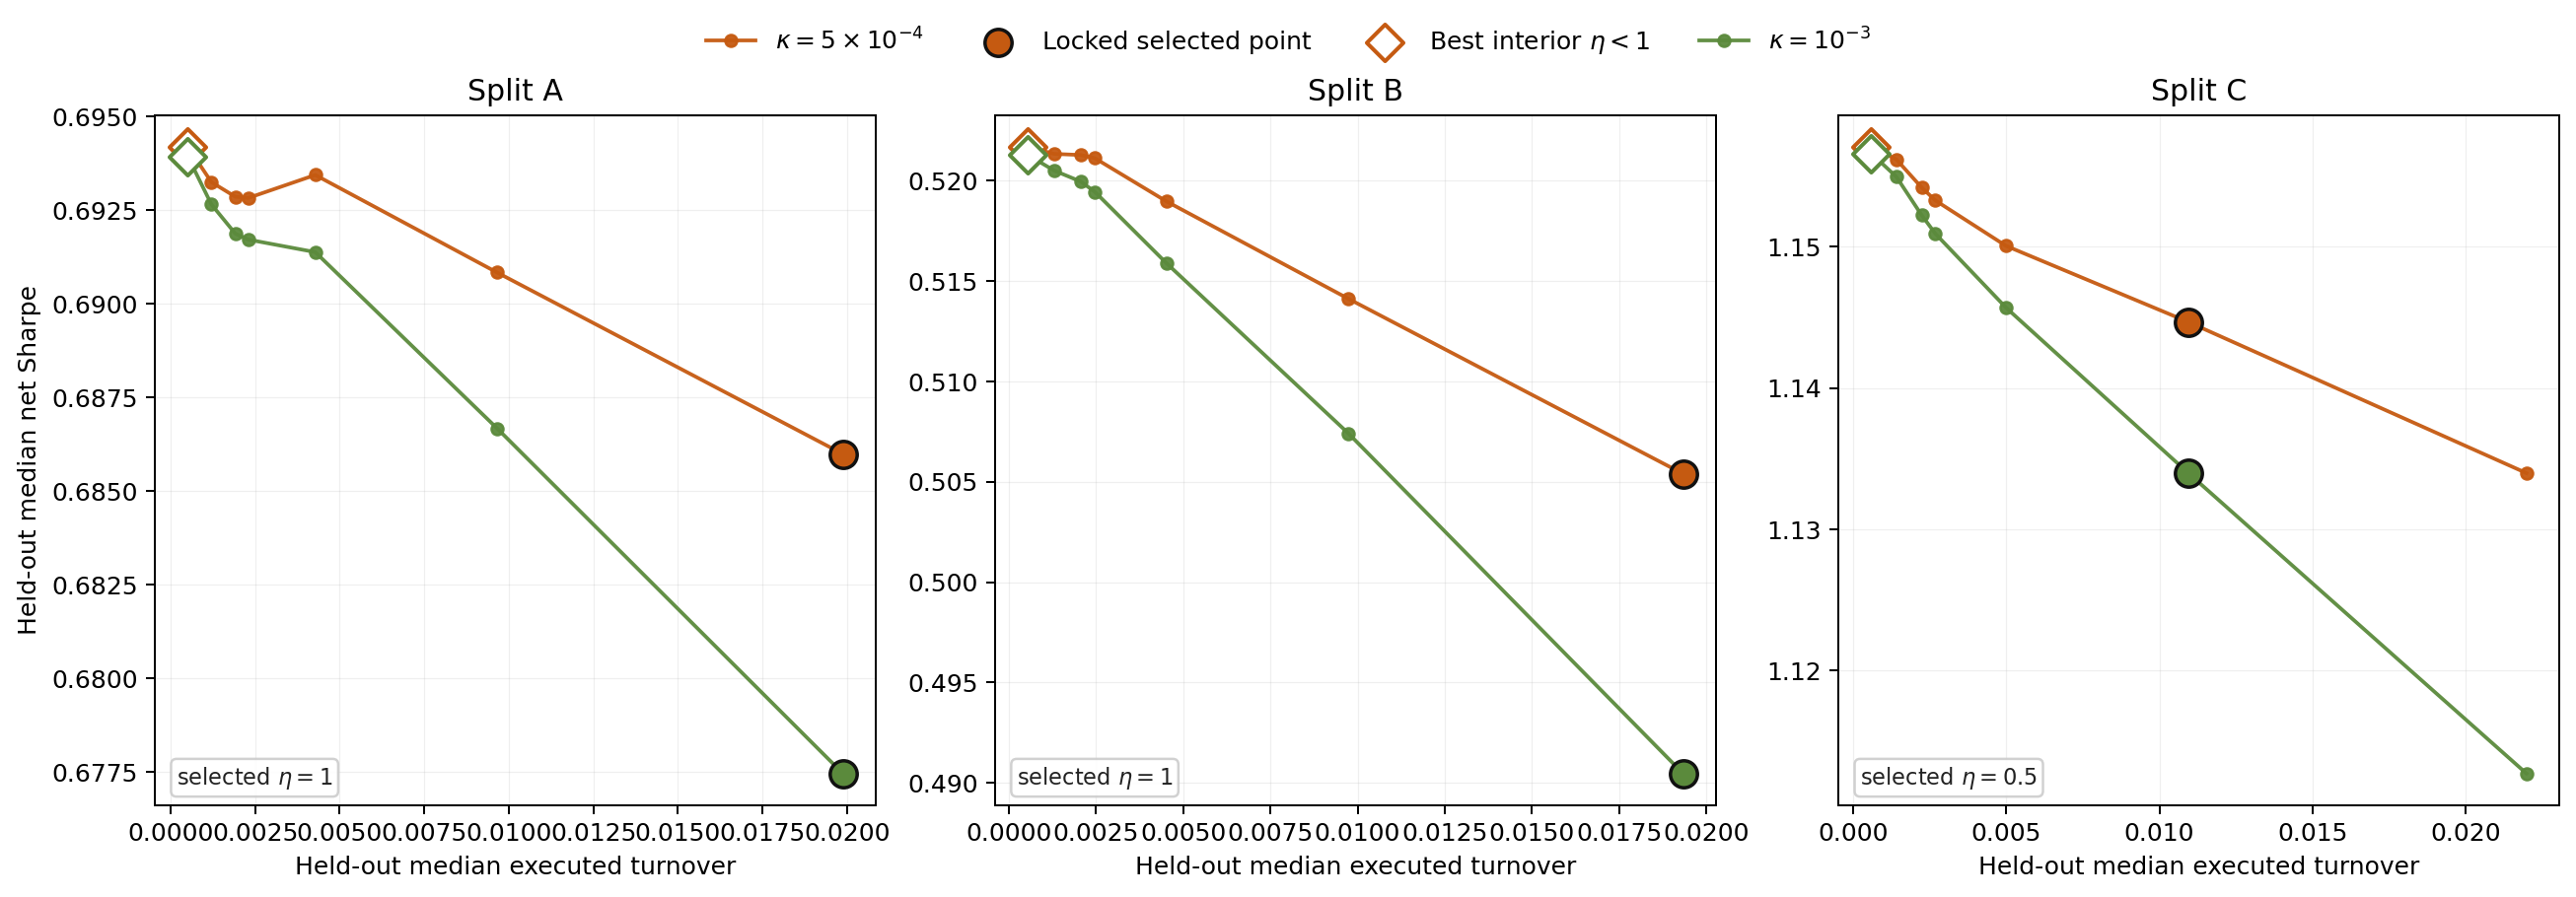
\includegraphics[width=0.92\textwidth]{fig_rolling_frontier_robustness.png}
\caption{Held-out positive-cost frontiers across the three rolling windows. Each panel shows the seed-median held-out net Sharpe versus seed-median executed turnover for $\kappa\in\{5\times10^{-4},10^{-3}\}$ over the fixed $\eta$ grid. Filled black-edged markers denote the locked validation-selected operating point for that split; hollow diamonds denote the best interior held-out point $\eta<1$, shown only as a post-selection diagnostic. Split C both selects and benefits from an interior point, whereas Splits A and B still exhibit interior frontiers even though the conservative selector remains at $\eta=1.0$.}
\label{fig:rollingfrontier}
\end{figure*}

\subsection{Denser friction grid: the frontier steepens as \texorpdfstring{$\kappa$}{kappa} grows}
We next densify the friction axis on the canonical split by adding $\kappa\in\{2\times10^{-4},2\times10^{-3}\}$ while keeping the frozen policy, the $\eta$ grid, and the validation-first protocol unchanged. This expansion is intentionally diagnostic: it does not retrain any policy and it does not replace the main selected-point result. Two findings are useful. First, the global validation selector remains stable. When positive costs are expanded to $\{2\times10^{-4},5\times10^{-4},10^{-3},2\times10^{-3}\}$, the same locked rule still selects $\eta=0.5$. Relative to immediate execution, that global selected operating point improves paired median net Sharpe by $+0.0041$, $+0.0105$, $+0.0213$, and $+0.0409$ as $\kappa$ increases across those four positive-cost regimes, while reducing median executed turnover by $0.01105$ in each row.

Second, the full held-out frontier becomes progressively more favorable to interior execution rates as friction grows. Using the best interior point only as a post-selection diagnostic, the paired median net-Sharpe gain versus $\eta=1.0$ rises monotonically from $+0.0113$ at $\kappa=2\times10^{-4}$ to $+0.0230$ at $\kappa=5\times10^{-4}$, $+0.0424$ at $\kappa=10^{-3}$, and $+0.0761$ at $\kappa=2\times10^{-3}$; the corresponding reduction in median executed turnover is essentially constant at about $0.02143$ because the comparison is always against the same immediate-execution baseline. A per-$\kappa$ diagnostic selector tells the same story from the other direction: it remains at $\eta=1.0$ for $\kappa=2\times10^{-4}$ and $5\times10^{-4}$, moves to $\eta=0.5$ at $\kappa=10^{-3}$, and tightens further to $\eta=0.2$ at $\kappa=2\times10^{-3}$. The friction-grid expansion therefore supports a simple interpretation: the execution frontier is not only real, but increasingly consequential as proportional trading frictions rise. Figure~\ref{fig:kappacurve} summarizes this tightening pattern across the dense friction grid.

\begin{figure*}[t]
\centering
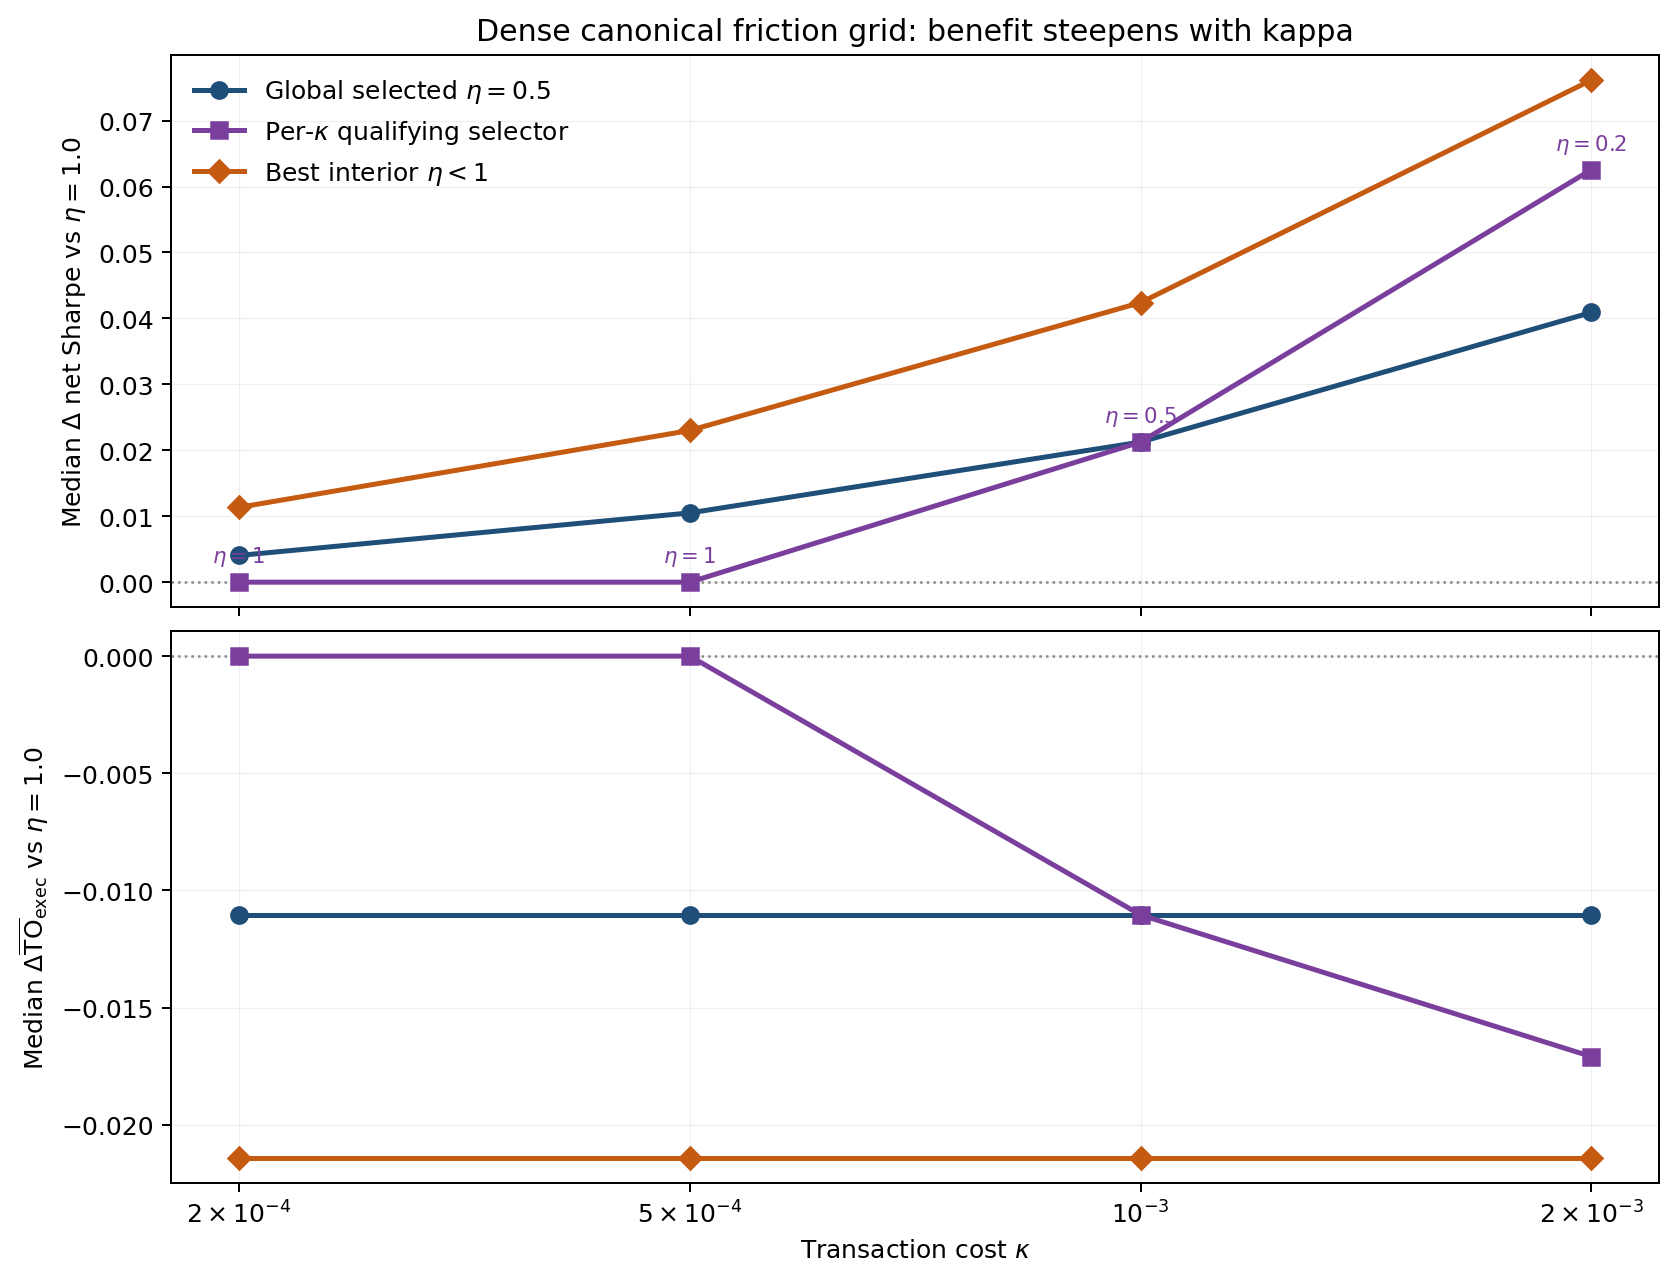
\includegraphics[width=0.80\textwidth]{fig_kappa_benefit_curve.png}
\caption{Dense canonical friction-grid benefit curve relative to immediate execution $\eta=1.0$. The top panel plots paired median $\Delta$ net Sharpe and the bottom panel plots paired median $\Delta\overline{\TOexec}$ on the held-out 2024--2025 split as $\kappa$ increases from $2\times10^{-4}$ to $2\times10^{-3}$. The blue line is the global validation-selected operating point $\eta=0.5$, the purple line is the per-$\kappa$ qualifying selector, and the orange line is the best interior held-out point $\eta<1$ shown only as a diagnostic. The per-$\kappa$ selector annotations show how the conservative operating point moves inward only once frictions become large enough, while the best-interior Sharpe gain steepens monotonically with $\kappa$.}
\label{fig:kappacurve}
\end{figure*}

\FloatBarrier
\subsection{Adaptive \texorpdfstring{$\eta_t$}{eta-t} schedules are out of scope}
Adaptive schedules are intentionally left out of the present version. The goal of this paper is to isolate the execution effect under a single frozen control model; adding rule-based $\eta_t$ schedules would mix execution design with schedule-selection effects. We therefore treat adaptive execution as future work and use the fixed-$\eta$ frontier as the main empirical object.

% ============================================================
\section{Discussion}
\paragraph{Interpretation: realized-path stabilization, not alpha creation.}
The central empirical result is not that a different prediction model has been learned, but that the same learned target path can be implemented in a more cost-aligned way under frictions. On the canonical 2024--2025 split, moving from immediate execution to the validation-selected interior operating point $\eta=0.5$ roughly halves median executed turnover and improves net Sharpe in the positive-cost regimes, while the corresponding gross-Sharpe change is slightly negative. The resulting interpretation is therefore narrow and mechanistic: under a fixed learned policy, execution-aware control improves risk-adjusted performance primarily through lower realized turnover and lower realized cost, not through additional predictive alpha.

\paragraph{When and why does execution help most?}
The evidence also clarifies when execution control matters most. First, its gains are concentrated in positive-cost regimes: on the canonical split, paired median net-Sharpe improvements are $+0.0105$ at $\kappa=5\times10^{-4}$ and $+0.0213$ at $\kappa=10^{-3}$, whereas the $\kappa=0$ result is negligible. Second, the selected interior operating point produces a substantial reduction in executed turnover while maintaining only modest target--executed mismatch. Third, on the denser canonical friction grid, the best interior held-out gain steepens monotonically with $\kappa$, indicating that the execution frontier becomes more consequential as frictions rise. Taken together, these patterns support a friction-sensitive stabilization view rather than a broad claim that smaller $\eta$ is universally better.

\paragraph{Rolling-window diagnostic.}
The rolling-window diagnostic should be read carefully. It does not show that one conservative validation-selected operating point transfers unchanged across windows. In two additional windows, the locked selector remained at $\eta=1.0$ because immediate execution stayed sufficiently close to the split-wise validation best. What persists more robustly is not selected-point transfer, but frontier existence: across all three windows, the positive-cost held-out frontier still contains interior execution rates that improve net Sharpe while lowering executed turnover relative to $\eta=1.0$. The rolling-window result therefore acts less as a broad robustness win than as a boundary condition on when conservative validation selection activates smoothing.

\paragraph{Matched heuristics as context only.}
The matched heuristic baselines provide only secondary context. Under aligned executed-path accounting, the selected operating point is competitive against several higher-churn comparators such as inverse-volatility risk parity and minimum-variance, mixed against daily-rebalanced equal weight and long-only mean-variance, and weaker than buy-and-hold equal weight on this window. These results help locate the empirical scale of the effect, but they do not define the paper's main claim, which remains the internal frozen-policy execution comparison.

\paragraph{Limitations.}
The limitation structure mirrors the contribution structure. The paper contributes executed-path accounting, a fixed-$\eta$ execution frontier analysis, and a frozen-policy empirical study. The present evidence is therefore bounded by the market abstraction used for accounting, the fixed-timescale design, and the absence of retraining comparisons.
\begin{itemize}[leftmargin=*,itemsep=1pt]
\item The executed-path accounting contribution is established under a daily close-to-close abstraction on a fixed 27-name large-cap U.S. equity snapshot with a no-cash long-only simplex. These choices make the accounting object transparent, but they also limit market realism and leave survivorship-related bias unresolved.
\item The execution-mapping contribution is established only for fixed $\eta$ schedules. Adaptive schedules and richer execution-control laws are intentionally excluded so that execution design is not confounded with schedule-selection effects.
\item The empirical contribution isolates execution under one frozen control model. Its strongest selected-point transfer result appears on the canonical split, while the rolling-window diagnostic shows that frontier existence is more robust than conservative selected-point transfer. Training-time alignment and retraining comparisons remain outside the scope of this version.
\item Secondary heuristic comparisons are reported under aligned accounting only as matched context. Comparator breadth is not a main contribution of this version, and broader classical comparisons are left to follow-on work.
\end{itemize}

% ============================================================
\section{Conclusion}
We formulate execution-aware portfolio reinforcement learning by separating target and executed portfolios and attaching both trading costs and primary evaluation to the realized executed path. Empirically, one trained policy is reused throughout, only the execution mapping varies over a fixed \emph{a priori} $\eta$ grid, $\eta$ is selected on validation only, and the test split is reserved for held-out evaluation.

On the canonical 2022--2025 split, the validation-selected operating point $\eta=0.5$ roughly halves median executed turnover and improves paired median net Sharpe in both positive-cost regimes, while the $\kappa=0$ evidence remains negligible. Across three rolling windows, the positive-cost held-out frontier remains interior even when conservative selected-point transfer does not persist. On a denser canonical friction grid, the same global selected operating point remains $\eta=0.5$, while the best interior held-out gain increases monotonically with friction. Mechanistically, these gains are explained by lower realized turnover and lower realized cost rather than by improved gross Sharpe.

Under a fixed learned trading policy, cost-aligned execution control creates an interior positive-cost execution frontier whose gains are driven primarily by lower realized turnover and lower realized cost, while selected-point transfer remains window-sensitive. This version is limited to frozen-policy identification rather than retraining comparisons, broad benchmark dominance claims, or deployment-grade point-in-time backtesting. Future work should focus on explicit training-time alignment comparisons, broader comparator studies, and adaptive execution schedules built on top of this locked frozen-policy protocol.

% ============================================================
\clearpage
\onecolumn
\appendix
\section{Reproducibility Checklist}
\label{app:repro}
\begin{itemize}[leftmargin=*,itemsep=1pt]
\item Paired-seed evaluation across all arms.
\item Per-run config archiving and command logging.
\item Environment signature files to detect drift.
\item Automated aggregation outputs (tables/figures) generated from stored traces.
\item Hard-locked core definitions: \eqref{eq:exec_update}--\eqref{eq:reward}.
\end{itemize}

\section{Data and Protocol Clarifications}
\label{app:data_protocol}
\subsection{Fixed universe, cache, and adjusted-close data}
The paper rebuild uses a cache-only paper-mode snapshot built from daily adjusted close prices retrieved via \texttt{yfinance}. Adjusted close is used so that stock splits and dividend adjustments are reflected in the return series rather than treated as spurious price jumps. The processed cache for the locked run is the fixed directory \texttt{data/processed\_u27}, and the frozen training config uses a fixed-list universe with 27 assets:

\begin{quote}
\small\ttfamily
AAPL, AMGN, AXP, BA, CAT, CRM, CSCO, CVX, DIS, GS, HD, HON, IBM, INTC, JNJ, JPM, KO, MCD, MMM, MRK, MSFT, NKE, PG, UNH, V, VZ, WMT
\end{quote}
This is a reproducible fixed 27-name snapshot, not a historical point-in-time constituent reconstruction. Legacy project naming may still contain ``Dow30'', but the locked paper rebuild uses the fixed 27-name universe listed above. Accordingly, the empirical protocol should be interpreted as a controlled benchmark study with survivorship-related limitations, not as a deployment-grade backtest free of constituent-selection bias.

\subsection{Decision timing and return interval}
The backtest uses a close-to-close convention. At decision time $t$:
\begin{enumerate}[leftmargin=*,itemsep=1pt]
\item the state $s_t$ is built only from information available up to close $t$,
\item the policy outputs the target portfolio $\wtgt_t$,
\item the execution controller forms the executed portfolio $\wexec_t$ via \eqref{eq:exec_update},
\item transaction cost is charged on executed turnover $\TOexec_t$ via \eqref{eq:cost_exec},
\item the realized return applied to the portfolio is the next-period close-to-close return over $(t,t+1]$.
\end{enumerate}
Thus the paper uses the convention ``decide at close $t$, then hold $\wexec_t$ over $(t,t+1]$.'' This ordering is important because both return realization and cost accounting are attached to the executed portfolio rather than to the raw target action.

\subsection{Anti-lookahead timing schematic}
The timing logic can be summarized as
\[
\text{state through close } t
\;\rightarrow\;
\wtgt_t
\;\rightarrow\;
\wexec_t
\;\rightarrow\;
\kappaTC \TOexec_t
\;\rightarrow\;
\text{hold over }(t,t+1]
\;\rightarrow\;
R_{t+1}.
\]
This schematic is the implementation counterpart of the formal definitions in Section~\ref{sec:setup}: the target portfolio is proposed at time $t$, the execution layer forms the realized holdings, costs are charged on executed turnover, and only then is the next-period return realized.

\subsection{Frozen split and model-selection lock}
The locked rebuild materializes the experiment configuration before evaluation. The train, validation, and held-out test windows are frozen as 2010--2021, 2022--2023, and 2024--2025, respectively. Because the state uses 30-day rolling features, the realized validation/test traces begin on 2022-02-15 and 2024-02-14 inside those split boundaries. The selected signal snapshot is also frozen before validation and test evaluation; in the rebuilt run, the frozen signal list is \texttt{reversal\_5d} and \texttt{short\_term\_reversal}. The $\eta$ grid is fixed \emph{a priori}, validation selects one operating point, and the test window is then used only for final evaluation of that selected operating point and matched comparators. Internal forward checks for 2026 were used only for engineering sanity and are not included in the paper tables or in $\eta$ selection.

\subsection{Constraint set and omitted assets}
All experiments use a long-only, fully invested simplex. In particular, portfolio weights are constrained to be non-negative and to sum to one each period. The present study does not include an explicit cash asset, leverage, or short positions. This means that the execution controller studies the effect of partial adjustment within a risky-asset simplex only. The no-cash design is intentional for interpretability, but it also limits the strategy class and should be read as a scope restriction rather than as a claim about the best practical trading interface.

\subsection{Backtest scope limitations}
The protocol is designed to be reproducible and internally consistent, but its scope remains limited in several ways:
\begin{itemize}[leftmargin=*,itemsep=1pt]
\item fixed 27-name large-cap U.S. equity snapshot rather than point-in-time constituent reconstruction,
\item no explicit cash asset,
\item long-only fully invested simplex,
\item daily close-to-close execution abstraction rather than intraday microstructure modeling,
\item frozen-policy empirical scope rather than a full retraining comparison.
\end{itemize}
These limitations do not invalidate the execution-accounting contribution, but they do bound the external claims that should be made from the current experiments.

\section{Implementation Details}
\label{app:implementation_details}
\subsection{Observation and action instantiation}
\begin{itemize}[leftmargin=*,itemsep=1pt]
\item Data source and cache: daily adjusted close prices retrieved via \texttt{yfinance} are materialized once and then reused in cache-only paper mode for training and evaluation.
\item Universe treatment: the paper rebuild uses the fixed 27-name snapshot rather than a point-in-time constituent reconstruction.
\item Observation schema: $L=30$ return history, $L_v=30$ volatility features, previous executed weights, and two signal channels (\texttt{reversal\_5d}, \texttt{short\_term\_reversal}).
\item Observation dimension: for 27 assets, the instantiated observation size is $30\times27 + 27 + 27 + 2\times27 = 918$, matching the stored run metadata.
\item Action parameterization: the actor emits one real-valued logit per asset; the environment clips the action vector to $[-1,1]$ and maps it to the simplex with a stable softmax using logit scale 10.0.
\end{itemize}

\subsection{Frozen controller configuration}
\begin{itemize}[leftmargin=*,itemsep=1pt]
\item RL backend: Stable-Baselines3 SAC (\texttt{sb3\_version}=2.7.1 in the stored metadata).
\item SAC hyperparameters: learning rate $10^{-4}$, batch size 256, discount $\gamma=0.99$, target-update rate $\tau=0.005$, replay buffer size 100000, total timesteps 100000, entropy coefficient 0.2.
\item PRL scheduler parameters: $\alpha_0=0.2$, $\beta=1.0$, $\lambda_v=2.0$, bias $=-2.0$, $\alpha_{\min}=0.01$, $\alpha_{\max}=1.0$, mid-plasticity multiplier 0.7, CVaR-penalty gamma 0.3.
\item Frozen signals: \texttt{reversal\_5d} and \texttt{short\_term\_reversal}, loaded from the locked selected-signals snapshot.
\end{itemize}

\subsection{Execution-grid provenance}
\begin{itemize}[leftmargin=*,itemsep=1pt]
\item The evaluation grid is fixed to $\eta\in\{1.0, 0.5, 0.2, 0.1, 0.082, 0.05, 0.02\}$ before validation and test evaluation.
\item The value $\eta=0.082$ is not a post-hoc insertion: it is the incumbent \texttt{rebalance\_eta} stored in the frozen control snapshot used to train the reference policy.
\item Validation selects one operating point from that fixed grid, and the held-out test split is then reserved for final evaluation only.
\end{itemize}

\section{Secondary Matched-Heuristic Context}
\label{app:secondary_heuristics}
Table~\ref{tab:selected_vs_external} is reported only as secondary context and is not part of the main identification strategy. Under the same effective held-out dates, the same transaction-cost definition $\kappaTC\cdot\TOexec$, the same annualization $\sqrt{252}$, and the same $r_f=0$ convention, the selected operating point is stronger than inverse-volatility risk parity and minimum-variance, mixed against daily-rebalanced equal weight and long-only mean-variance, and weaker than buy-and-hold equal weight on this window. These matched heuristics help calibrate the empirical scale of the result under aligned accounting, but they do not define the paper's main claim and they do not change the frozen-policy interpretation of the internal execution frontier.

\begin{center}
\captionsetup{type=table}
\captionof{table}{Held-out test comparison between the validation-selected operating point $\eta=0.5$ and matched heuristic baselines on the effective held-out dates 2024-02-14 to 2025-12-31 within the 2024--2025 split. All quantities use the same executed-path accounting conventions.}
\label{tab:selected_vs_external}
\scriptsize
\begin{tabular}{@{}llrrrrr@{}}
\toprule
$\kappaTC$ & Baseline & Baseline Sharpe & $\Delta$Sharpe & Baseline CAGR & $\Delta$CAGR & $\Delta\overline{\TOexec}$ \\
\midrule
$0$ & Buy-and-hold EW & 1.1726 & -0.0172 & 0.1651 & -0.0001 & +0.01095 \\
$0$ & Daily-rebalanced EW & 1.1530 & +0.0024 & 0.1646 & +0.0004 & +0.00106 \\
$0$ & Inverse-vol RP & 1.0772 & +0.0782 & 0.1416 & +0.0234 & -0.02210 \\
$0$ & Minimum-variance & 1.0649 & +0.0905 & 0.1219 & +0.0431 & -0.04160 \\
$0$ & Mean-variance (long-only) & 1.2269 & -0.0716 & 0.1841 & -0.0190 & -0.08780 \\
$5\times10^{-4}$ & Buy-and-hold EW & 1.1726 & -0.0279 & 0.1651 & -0.0018 & +0.01095 \\
$5\times10^{-4}$ & Daily-rebalanced EW & 1.1441 & +0.0005 & 0.1632 & +0.0001 & +0.00106 \\
$5\times10^{-4}$ & Inverse-vol RP & 1.0453 & +0.0994 & 0.1369 & +0.0264 & -0.02210 \\
$5\times10^{-4}$ & Minimum-variance & 1.0064 & +0.1382 & 0.1145 & +0.0487 & -0.04160 \\
$5\times10^{-4}$ & Mean-variance (long-only) & 1.1420 & +0.0027 & 0.1694 & -0.0061 & -0.08780 \\
$10^{-3}$ & Buy-and-hold EW & 1.1726 & -0.0386 & 0.1651 & -0.0035 & +0.01095 \\
$10^{-3}$ & Daily-rebalanced EW & 1.1353 & -0.0013 & 0.1617 & -0.0002 & +0.00106 \\
$10^{-3}$ & Inverse-vol RP & 1.0133 & +0.1206 & 0.1321 & +0.0294 & -0.02210 \\
$10^{-3}$ & Minimum-variance & 0.9480 & +0.1860 & 0.1072 & +0.0544 & -0.04160 \\
$10^{-3}$ & Mean-variance (long-only) & 1.0570 & +0.0770 & 0.1550 & +0.0066 & -0.08780 \\
\bottomrule
\end{tabular}
\par\vspace{2pt}\raggedright\footnotesize{\textit{Note:} All heuristic rows use the same effective held-out dates 2024-02-14 to 2025-12-31 and the same executed-path accounting conventions. Positive $\Delta\overline{\TOexec}$ means the selected RL arm trades \emph{more} than the comparator; negative values mean it trades less.}
\end{center}

\section{Supplementary Figures}
\label{app:supp_figures}

\begin{center}
\captionsetup{type=figure}
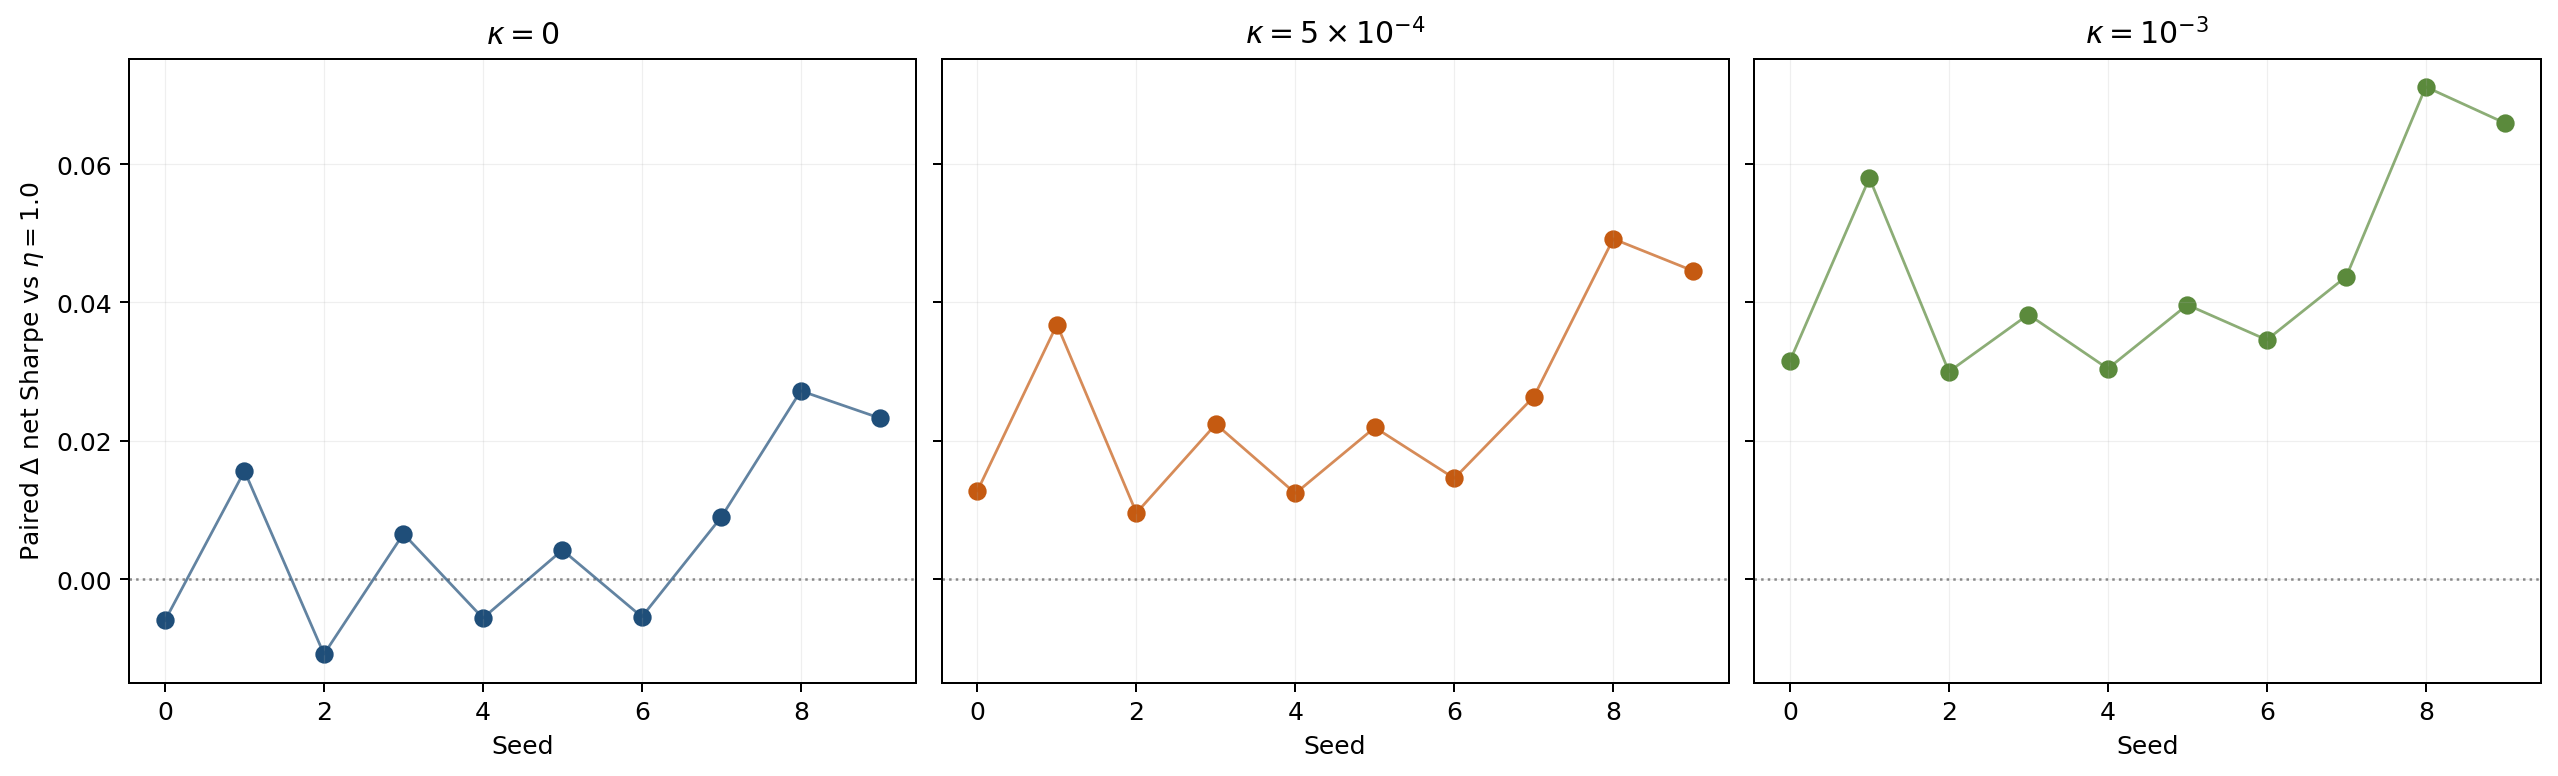
\includegraphics[width=0.88\textwidth]{fig_seed_scatter.png}
\captionof{figure}{Seed-wise paired $\Delta$ net Sharpe on the effective held-out dates 2024-02-14 to 2025-12-31 for the validation-selected operating point $\eta=0.5$ relative to the immediate-execution baseline $\eta=1.0$. This figure visualizes the same held-out paired comparison reported in Table~\ref{tab:selected_vs_eta1}. Each point is one seed-wise difference $\mathrm{Sharpe}_{\eta=0.5}-\mathrm{Sharpe}_{\eta=1.0}$, and the dotted horizontal line marks zero. All 10 paired seeds are positive in the two positive-cost regimes, matching the $10/10$ seed-win result reported in Table~\ref{tab:selected_vs_eta1}, whereas the $\kappa=0$ panel mixes positive and negative deltas.}
\label{fig:seedscatter}
\end{center}

\begin{center}
\captionsetup{type=figure}
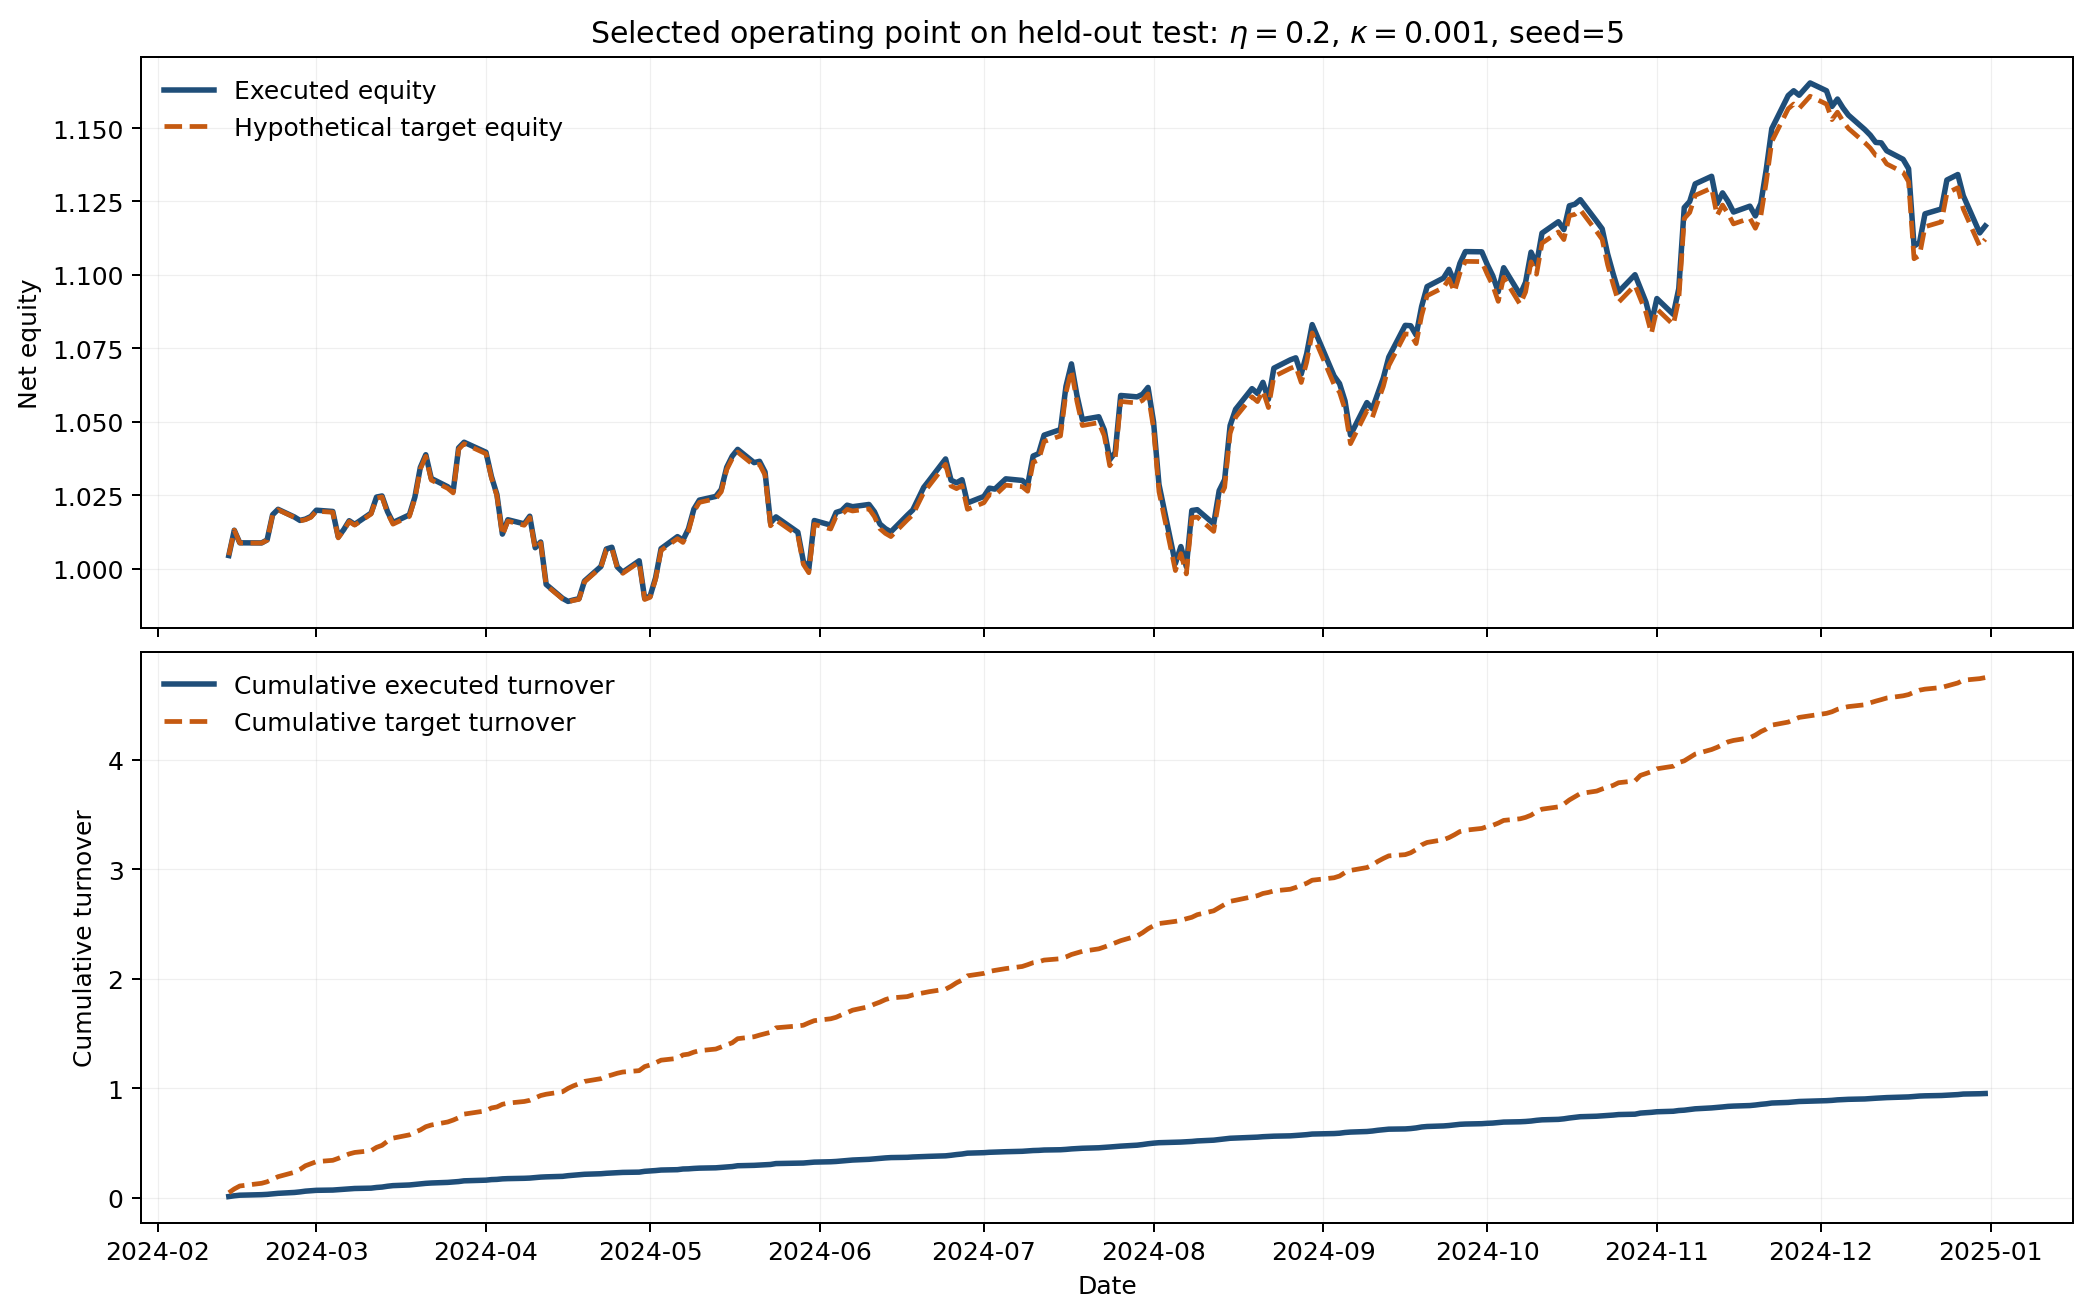
\includegraphics[width=0.92\textwidth]{fig_misalignment.png}
\captionof{figure}{Representative held-out trace for the validation-selected operating point on the effective held-out dates 2024-02-14 to 2025-12-31 within the 2024--2025 split at $\eta=0.5$, $\kappa=10^{-3}$, seed 2. The top panel shows executed net equity and hypothetical target net equity, where the target path is the immediate move to the target portfolio used only for diagnostics. The bottom panel shows cumulative executed and target turnover. The representative seed is the selected-arm run whose held-out net Sharpe is closest to the median selected-arm net Sharpe across the 10 paired seeds at $\kappa=10^{-3}$.}
\label{fig:misalign}
\end{center}

% ============================================================
\begin{thebibliography}{99}
\bibitem{markowitz1952}
H. Markowitz, ``Portfolio Selection,'' \emph{The Journal of Finance}, 1952.

\bibitem{merton1973}
R. C. Merton, ``An Intertemporal Capital Asset Pricing Model,'' \emph{Econometrica}, 1973.

\bibitem{bertsimas1998}
D. Bertsimas and A. W. Lo, ``Optimal Control of Execution Costs,'' \emph{Journal of Financial Markets}, 1998.

\bibitem{moody1998}
J. Moody and M. Saffell, ``Learning to Trade via Direct Reinforcement,'' \emph{IEEE Transactions on Neural Networks}, 1998.

\bibitem{jiang2017}
Z. Jiang, D. Xu, and J. Liang, ``A Deep Reinforcement Learning Framework for the Financial Portfolio Management Problem,'' \emph{CoRR}, abs/1706.10059, 2017.

\bibitem{nevmyvaka2006}
Y. Nevmyvaka, Y. Feng, and M. Kearns, ``Reinforcement Learning for Optimized Trade Execution,'' \emph{Proceedings of the 23rd International Conference on Machine Learning}, 2006.

\bibitem{ye2020}
Y. Ye, H. Pei, B. Wang, P.-Y. Chen, Y. Zhu, J. Xiao, and B. Li, ``Reinforcement-Learning Based Portfolio Management with Augmented Asset Movement Prediction States,'' \emph{Proceedings of the AAAI Conference on Artificial Intelligence}, 34(1):1112--1119, 2020.

\bibitem{lien2023}
Y.-H. Lien, Y.-K. Li, and Y.-S. Wang, ``Contrastive Learning and Reward Smoothing for Deep Portfolio Management,'' \emph{Proceedings of the Thirty-Second International Joint Conference on Artificial Intelligence (IJCAI-23)}, pp. 3966--3974, 2023.

\bibitem{lobo2007}
M. Lobo, M. Fazel, and S. Boyd, ``Portfolio Optimization with Linear and Fixed Transaction Costs,'' \emph{Annals of Operations Research}, 152(1):341--365, 2007.

\bibitem{li2014}
B. Li and S. C. H. Hoi, ``Online Portfolio Selection: A Survey,'' \emph{ACM Computing Surveys}, 2014.

\bibitem{garleanu2013}
N. G\^arleanu and L. H. Pedersen, ``Dynamic Trading with Predictable Returns and Transaction Costs,'' \emph{The Journal of Finance}, 68(6):2309--2340, 2013.

\bibitem{almgren2000}
R. Almgren and N. Chriss, ``Optimal Execution of Portfolio Transactions,'' \emph{Journal of Risk}, 3(2):5--39, 2000.

\bibitem{wang2021hrpm}
R. Wang, H. Wei, B. An, Z. Feng, and J. Yao, ``Commission Fee is not Enough: A Hierarchical Reinforced Framework for Portfolio Management,'' \emph{Proceedings of the AAAI Conference on Artificial Intelligence}, 35(1):626--633, 2021.

\bibitem{shen2020}
Q. Shen, Y. Li, H. Jiang, Z. Wang, and T. Zhao, ``Deep Reinforcement Learning with Robust and Smooth Policy,'' \emph{Proceedings of the 37th International Conference on Machine Learning}, \emph{PMLR} 119:8707--8718, 2020.

\bibitem{mysore2021}
S. Mysore, B. Mabsout, R. Mancuso, and K. Saenko, ``Regularizing Action Policies for Smooth Control with Reinforcement Learning,'' \emph{Proceedings of the IEEE International Conference on Robotics and Automation (ICRA)}, pp. 1810--1816, 2021.
\end{thebibliography}

\end{document}
